%\centerline{Christopher Guinnup; Sam Nixon; Bryan Schmier; Rui Xu; Mengjiao Han}
% CISC475: Advanced Software Engineering
% CISC675: Software Engineering Principles & Practices
% Template for software development project report

\documentclass[11pt]{report}
\usepackage[nottoc,numbib]{tocbibind}
\usepackage{graphicx}
\usepackage{caption}
\usepackage{subfigure}
\usepackage{color}
\usepackage{array}
\usepackage{float}
\usepackage{cite}
\usepackage{url}
\usepackage[letterpaper,textheight=9in,left=1in,%
textwidth=6.5in,bottom=1in]{geometry}
\usepackage{hyperref}
  
\title{Ping-pong Detection System}

\author{\textbf{Team 2}\\ 
  Christopher Guinnup, Rui Xu\\
  Sam Nixon, Mengjiao Han, Bryan Schmier\\
\\
  \emph{Client: Scott Kay}\\
  \emph{Professor: Stephen Seigel}
  % note: the titles are optional; if the members of your team
  % did not use any titles, don't put them here
}

% I put this macro here to make it easy to write glossary entries...
\newlength{\glosslen}
\setlength{\glosslen}{\textwidth}
\addtolength{\glosslen}{-10mm}
\newcommand{\gloss}[2]{
  \vspace{3mm}

  \noindent\textbf{#1}\vspace{1mm}

  \hspace{5mm}\parbox{\glosslen}{#2}}

% Put your own macros here...
\newcommand{\tabincell}[2]{\begin{tabular}{@{}#1@{}}#2\end{tabular}}


\begin{document}

\maketitle
\tableofcontents


\chapter{Preliminaries}

%%%%%%%%%%%%%%%  Change Log  %%%%%%%%% %%%%%
\section{Change Log}
\begin{center}

\begin{tabular}{|c|c|c|c|}\hline

Date & Changes & Author & Version\\\hline
9/8/14 & \tabincell{c}{Created document} & \tabincell{c}{Rui Xu\\Mengjiao Han} & 0.1\\\hline
9/16/14 & \tabincell{c}{1. Add EDR, DFD and the descriptions of them} & \tabincell{c}{Bryan Schmier}  &0.1\\\hline
9/19/14 & \tabincell{c}{1. Edit ERD, DFD \\2. Edit grammar mistakes} & \tabincell{c}{Bryan Schmier} & 0.1 \\\hline
10/1/14 & \tabincell{c}{1. Edit Overview\\2. Add Stakeholders\\3. Edit ERD, DFD and their descriptions\\4. Add Scope section\\5. Add Problem domain section\\6. Edit requirement section\\7. Add non-functional requirement section} &\tabincell{c}{Rui Xu\\Mengjiao Han\\Bryan Schmier} & 0.2\\\hline
10/3/14 &\tabincell{c}{1. Add the description of diagram\\ 2. Change grammar mistakes} &\tabincell{c}{Bryan Schmier} &0.2\\\hline
10/3/14 &\tabincell{c}{1. Added Design section\\2. Many editorial changes} &\tabincell{c}{Christopher Guinnup}& 0.2\\\hline
10/17/14 &\tabincell{c}{1. Changed Design section\\2. Many editorial changes\\3.Add verification plan} &\tabincell{c}{Christopher Guinnup\\Byran\\Mengjiao Han}& 0.3\\\hline
10/31/14 &\tabincell{c}{1. Major update to Design section} &\tabincell{c}{Christopher Guinnup} & 0.4\\\hline
10/31/14 & \tabincell{c}{1. Update to Verification section} &\tabincell{c}{Mengjiao Han} &0.4\\\hline
11/7/2014 & \tabincell{c}{1. Design: Added \texttt{computerVisionService}\\ submodules, \texttt{PDSMain},\\ cleaned up bad LaTeX syntax,\\positioned diagrams more logically.} &\tabincell{c}{Christopher Guinnup} & 0.5\\\hline
11/14/2014 & \tabincell{c}{1. Verification: Added Video Tests section\\ and performed \\misc proofreading and editing.} &\tabincell{c}{Christopher Guinnup} & 1.0\\\hline
\end{tabular}
\end{center}
\begin{center}
\begin{tabular}{|c|c|c|c|}\hline
12/4/2014 & \tabincell{c}{1. Design: Changed all names\\ to avoid abbreviations and\\ added the new Racket modules,\\ updated the diagrams, and misc revisions.} &\tabincell{c}{Christopher Guinnup} & 1.1\\\hline
\end{tabular}
\end{center}

%%%%%%%%%%%%%%   Introduction   %%%%%%%%%%%%%%%%
\section{Introduction}
At eMoney Company, there are several options when taking a break and relaxing with co-workers, but playing ping pong is the most popular one. The table is usually in high demand and thus results in long wait times. Workers need to check the status of the ping pong table to know whether the table is available. Moreover, the placement of this table will change sometimes. The purpose of this project is to automatically determine the status of the ping pong table by monitoring the table with a camera, and sending the availability status to employees by an external broadcast mechanism. This will prevent workers from walking to the recreation room in hopes of playing ping pong, only to find it already occupied.

Our project's name is Ping-Pong Detection System (PDS). Since the network video stream is not accessible outside of eMoney, PDS will use VLC media player(VLC) \cite{source1} to load videos already stored on a hard drive that have been recorded by the camera in the eMoney office. Since the project is part of a whole system, the output will be messages texted in console. eMoney will make more extensions based on PDS's results.
Our team's name is ``The Twisted Platypi" and our members are Christopher Guinnup, Sam Nixon, Bryan Schmier, Mengjiao Han and Rui Xu. The URL of our team is \mbox{\url{http://cisc475-2.cis.udel.edu/}}. We use SVN as our version control tool, and the full repository is at \mbox{\url{svn://cisc475-2.cis.udel.edu/twistpong}}. We also use Trac to track and manage the project's tasks and issues. The main page of Trac is \mbox{\url{http://cisc475-2.cis.udel.edu/trac/twistpong/}}. And the documents in the project will be prepared by LaTeX. 

% Chris Guinnup comment: The Table of Contents already describes the document, it's considered poor form to redundantly spell it out in the text.

% This document describes PDS and has 3 chapters. The first chapter is preliminaries, which shows the change log of this document and a brief introduction of our project. The second chapter is requirements, which details the different requirements of the project. The third chapter is design, which presents the basic architecture of the system and some detailed designs regarded entities relationships and data flow. The glossary and the bibliography are presented on the appendix.

%%%%%%%%%%%%%  Requirement    %%%%%%%%%%%%%%%%%%%%%%
\chapter{Requirements}

\section{Stakeholders}

(1)	Employees of eMoney: Need a notification to let them know whether the ping pong table is available for play or not.  They would also prefer not to be misled by a false result from our system.  Some employees may not like the idea of software analyzing recreation room video, and may try to turn the camera away.\\
(2)	Client Scott Kay: Would like us to deliver the software on time and in a way that fits his company's setup.\\

% Chris Guinnup comment: Do **NOT** copy whole passages of text from a document you didn't work on, while giving no credit to the author! This is called plagarism, a serious offense which can result in severe academic punishment.

% (3)	Professor Siegel: Needs the system complexity to be kept at a level where students have a reasonable chance to complete the project within the time frame of the semester. He also needs the system to be complex enough for students to get experience with real world software issues.\\
% (4)	Students of CISC475/765 (Fall 2014): Need the system to be complex enough to accurately represent how software engineering works in the real world.

\section{Scope}

We will design a program that takes video as input, which includes recordings of the table during different states of vacancy, and then output the status of the table. Our program will rely on a library (currently the VLC media player library) for receiving video and decoding the compressed format. We have been provided with sample videos which were filmed at the eMoney office. In these videos, the angle of the camera, the status of the table (in use or not), and even the color of the ball are all different. Our program's goal is to handle these different conditions, and output the status of the ping pong table. The output will be textual, to a single console, and includes (1) ``Ping pong game is in progress", (2) ``The ping pong table is available", (3) ``Camera no longer pointing at the table".  The client will integrate this output into a broadcast system of their own.

\section{Problem Domain}
(1)	Console: Will display the result of the PDS. As PDS is part of a whole system at eMoney, they will make extensions based on these results, like linking to Twitter.\\
(2)	Table: The ping pong table which eMoney employees play on. The table is a regular dark green ping pong table with white edges, which has two sides divided by a net.  The table could be moved, or it may be partially obscured by players at certain times.\\
(3)	Camera: The input device; it records clear video of the table and transfers the video to the PDS to analyze. There are different angles between the camera and the table. The captures of videos are in Figure 2.1. Ideally, the camera is shooting vertically at the table. And in this case, the video's screen will all fill with the ping pong table. However, sometimes the camera could be at a different angle. In this case, the video's screen will only fill some part of the table.\\
%%%%%%%%%  Figure 2.1: the capture of videos  %%%%%%%%%%%%%%%%
\begin{figure}[float]
\centering
\subfigure{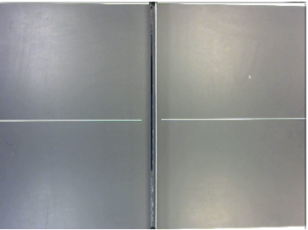
\includegraphics[width=5cm,height=4cm]{ideal.png}}
\subfigure{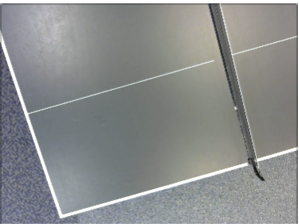
\includegraphics[width=5cm,height=4cm]{off-angle.png}}
\subfigure{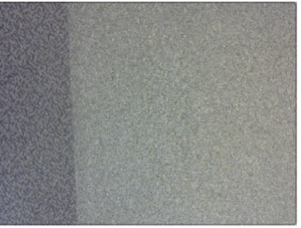
\includegraphics[width=5cm,height=4cm]{no-table.png}}
\caption{ \small{The captures of videos. (a) the ideal place of camera; (b) the different angle of camera; (c) the image when there is not a table.}}
\end{figure}
%%%%%%%%%%%%%%%%%%%%%%%%%%%%%%%%%%%%%%%%%%%
%\vspace{0.2cm}
(4)	Ball: The ping pong ball used by employees on the ping pong table. The ping pong ball is a regular ping pong ball and the color should not affect the result (although the color will most likely be white or orange).\\
(5)	Paddle: The ping pong paddle used for playing ping pong.\\
(6)	Lights: Lighting around the table is an average indoor situation, approximately 50,000 lumens for the 2,700 square foot room.\\
(7)	Playing environment: The environment around the ping pong table and tools for playing, including lighting, table, and ball.\\
(8)	Video: Frames of data recorded by the camera.

\section{Console}
In this section we will explain in detail the requirements of each different situation.\\

CS1. When user input the command to close the system, then the console will shut down.

CS2. While the system is running, the console will periodically update with one of three messages and a current time stamp. The messages are: 1) ``Ping pong game is in progress"; 2) ``The ping pong table is available"; 3) ``Camera no longer pointing at the table".

CS3. If no ball has moved for over 15 seconds, the console will display the message ``The ping pong table is available".

CS4. If a ball is moving across the table, the console will display the message ``Ping pong game is in progress".  During this state, the ball may go off screen, off the table, or become still on the table.  But as long as the ball stops for less than 15 seconds, the game is still considered in progress.

CS5. If the camera cannot detect the ping pong table, the console will text message ``Camera no longer pointing at the table".

CS6. If people are standing at the ping pong table but no balls are moving and no rackets are being waved around, the console will print message ``The ping pong table is available".

CS7. If people are standing at the ping pong table and waving rackets, the console will print message ``Ping pong game is in progress".  This status lasts until 5 seconds after they stop waving rackets.

CS8. When play ends, people may take the ball away or leave it on the table. No matter which situation appears, the result should still denote that the table is available.

CS9. When the state of the table or game has changed, the appropriate message will be printed as soon as this is detected.  If the state has not changed, any repeated message will be displayed after at least 15 seconds have passed.

\section{Video recording}
In this section we will explain in detail the requirements related to video recording.\\

VR1. When the table is placed horizontally, the PDS should support all camera angles from 30 to 150 degrees, as Figure 2.2 .
%%%%%%%%   Figure 2.2 The angle of the camera %%%%%%%%%%%%%%
\begin{figure}[!htb]
\centering
\subfigure{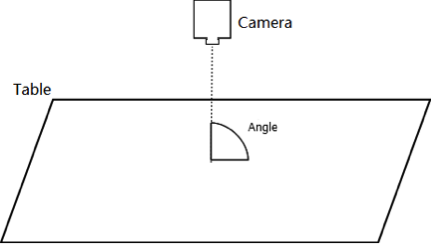
\includegraphics{VR1.png}}
\caption{ \small{ angles of the camera}}
\end{figure}
%%%%%%%%%%%%%%%%%%%%%%%%%%%%%%%%%%%%%%%%%%

VR2. When the table is rotated 90 degrees to face vertically, the PDS should support all camera angles from 30 to 150 degrees, as Figure 2.3.
%%%%%%%%   Figure 2.2 The angle of the camera %%%%%%%%%%%%%%
\begin{figure}[!htb]
\centering
\subfigure{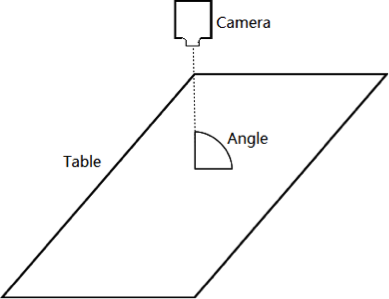
\includegraphics{VR2.png}}
\caption{ \small{angles of the camera}}
\end{figure}
%%%%%%%%%%%%%%%%%%%%%%%%%%%%%%%%%%%%%%%%%%

VR3.  MPEG2 and MPEG4 videos compression formats should be supported by the PDS.

VR4. The table could be moved, so not every video will have an entire ping pong table, as Figure 2.1(c) shows. If at least half the area of the table is in the video frame then the application should still function.

\section{General}
In this section we will explain the requirements related to the system in general.

G1. The application must have a very minimal error-rate (less than 10 percent), so that the employees can have an accurate and trustworthy indication of the table's availability.

G2. The system must be able to perform in real-time on modern computer hardware without a GPU.

\newpage
\section{Entity-Relationship Diagram}

In this section, we will describe the entity-relationship diagram of the project.\\

%%%%%%%%%%%  ER Diagram  %%%%%%%%%%%%%%%%%%%%%%%%
\begin{figure}[!htb]
\centering
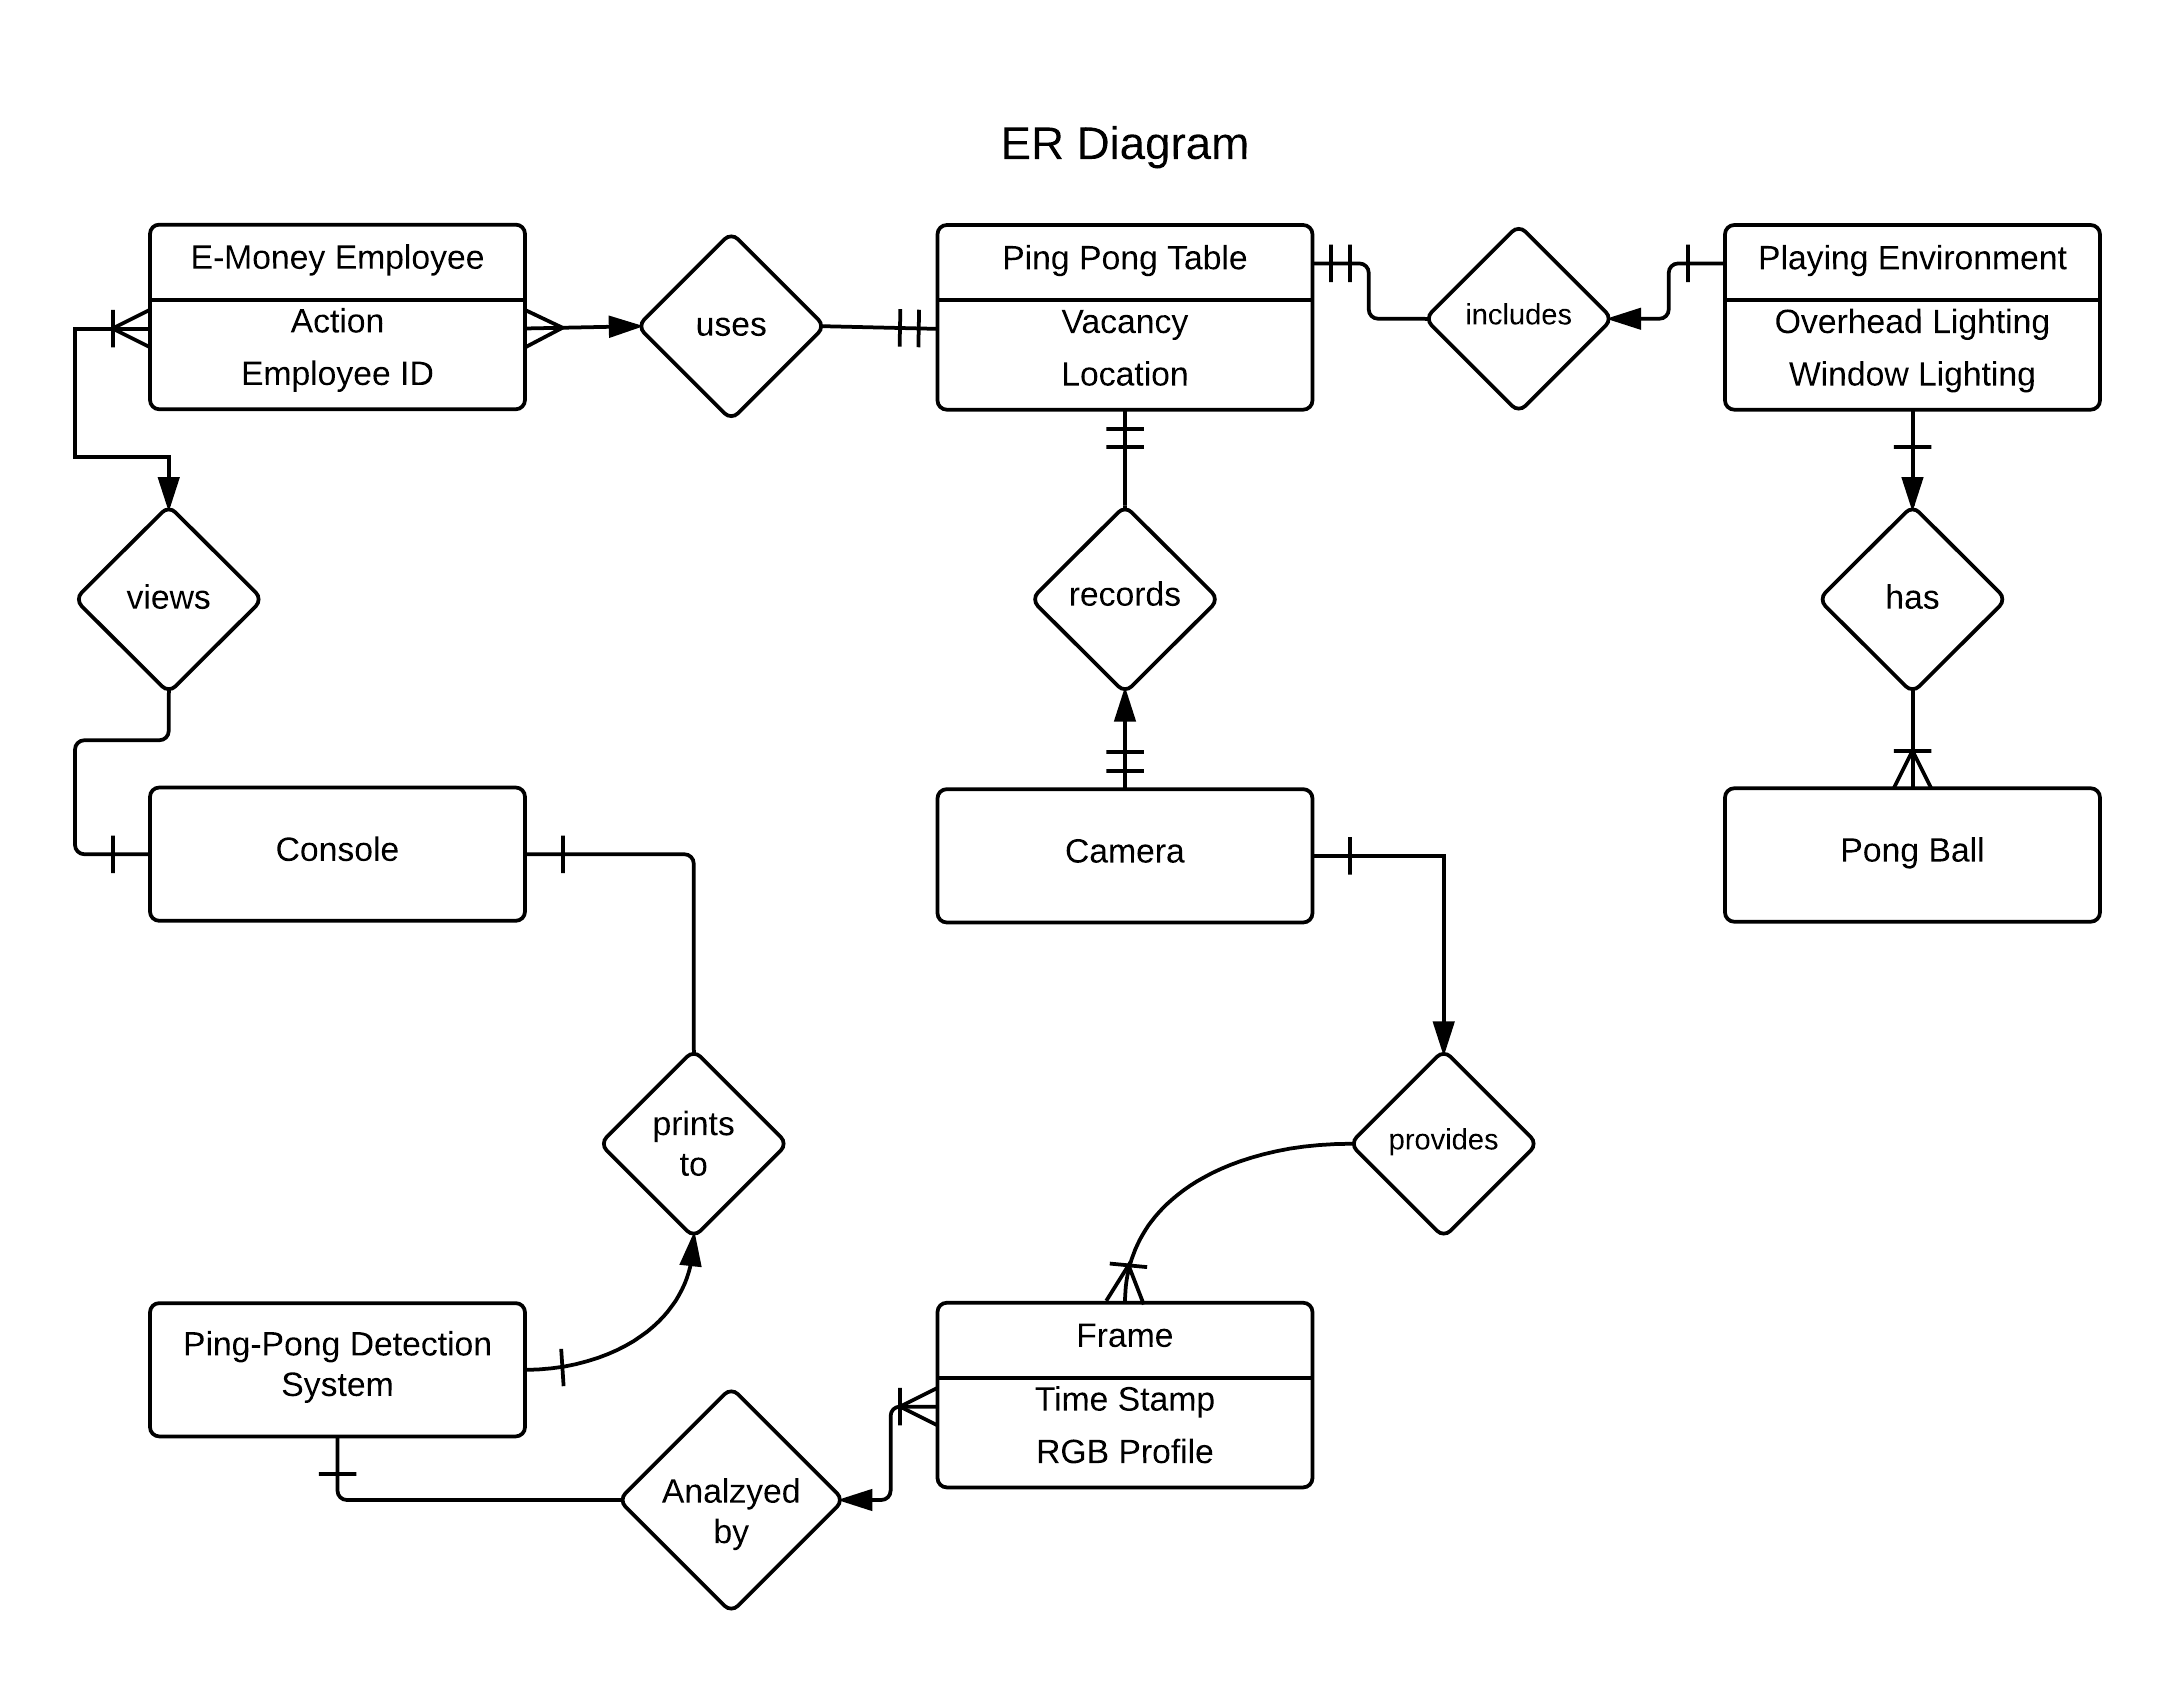
\includegraphics[width=1.05\textwidth]{ERDiagram2.png}

\caption{ \small{Entity-Relationship Diagram}}

\end{figure}
%%%%%%%%%%%%%%%%%%%%%%%%%%%%%%%%%%%%%%%%%
% add description
The ER Diagram shows each entity in our working system. Each eMoney Employee is always acting, whether its playing ping pong, checking the status of the table, or doing work. At the same time, the pong table with the factors of the environment are recorded by the camera which, in turn, creates a video feed for our program, the Ping-Pong Detection System (PDS). PDS then analyzes the video feed and sends the current availability status of the table to the console.

\newpage
\section{Data Flow Diagram}
%%%%%%%%%%%  Data Flow Diagram: Level 0  %%%%%%%%%%%%%%%%%%%%%%%%
\begin{figure}[!htb]
\centering
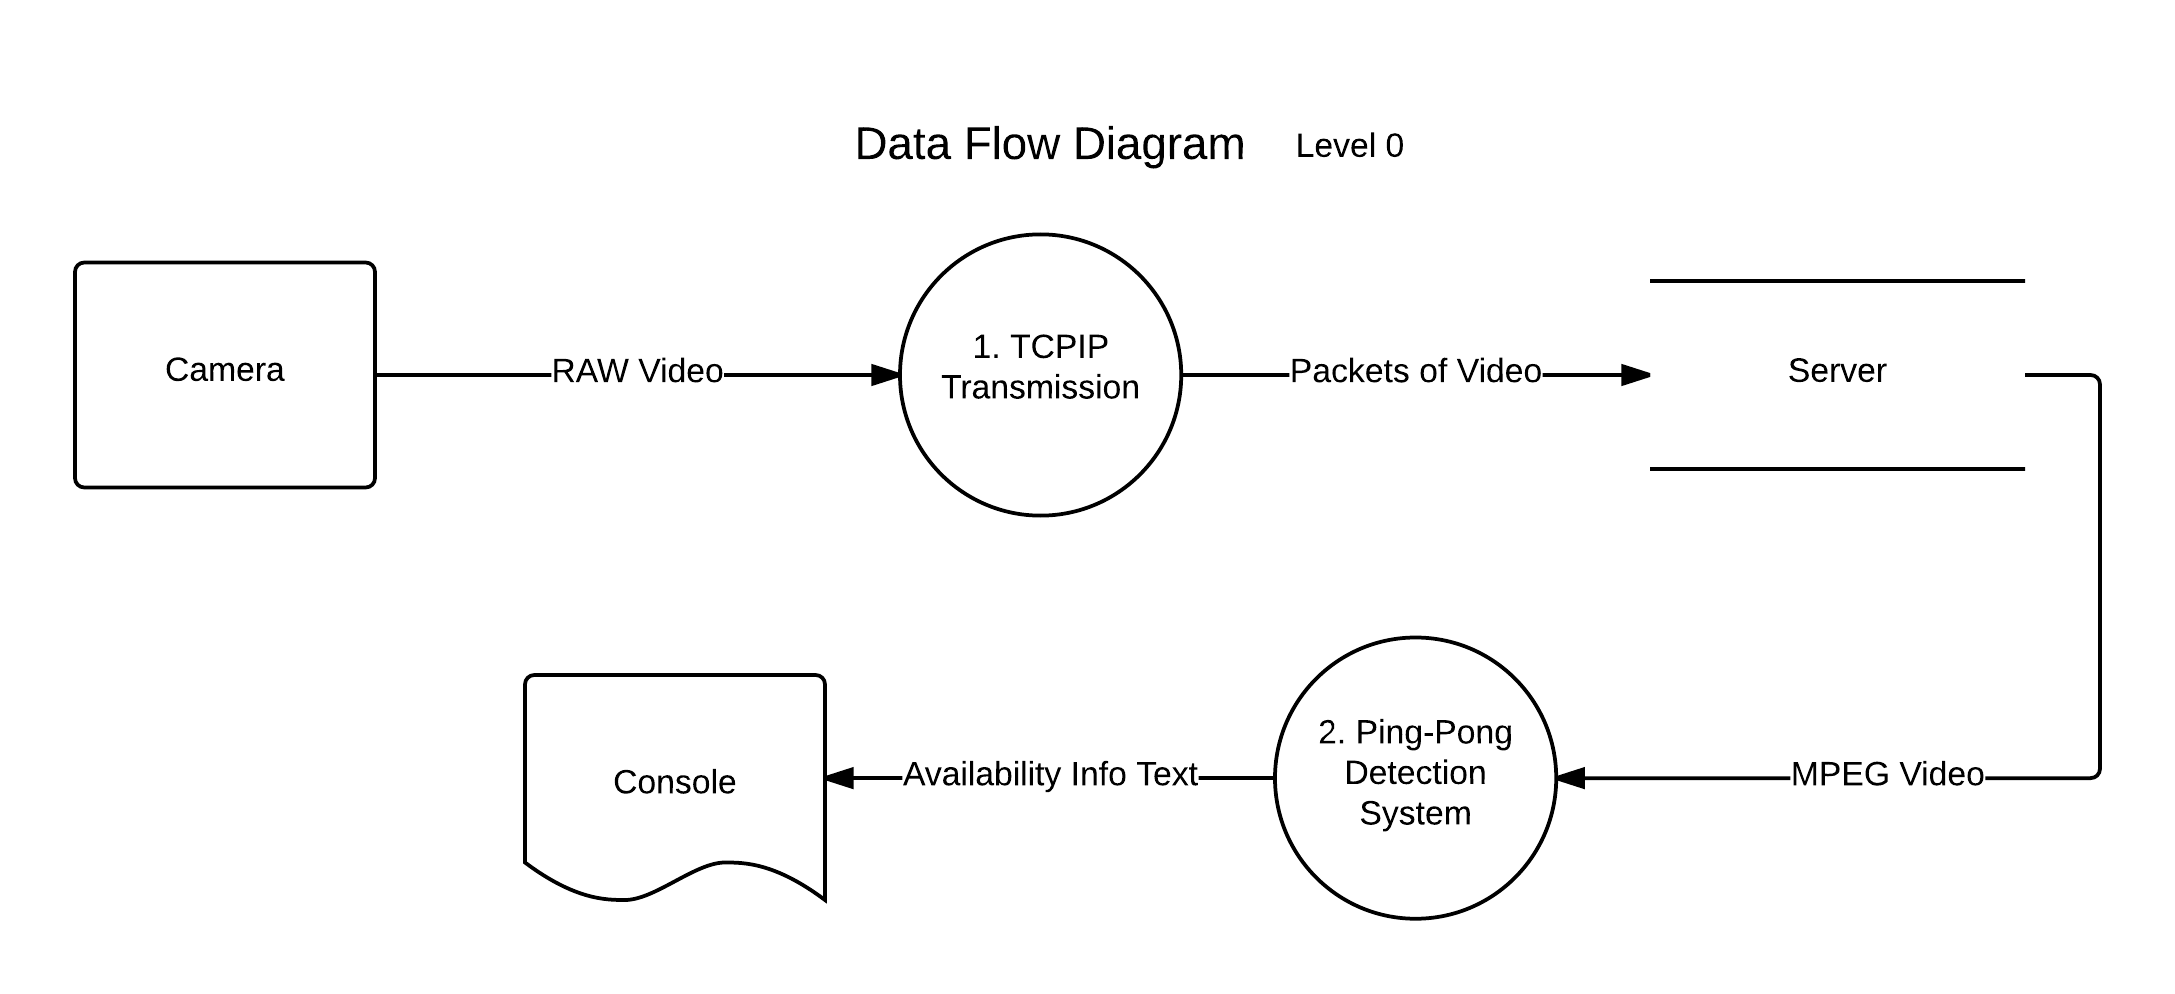
\includegraphics[width=1\textwidth]{Data-Flow-Level0.png}
\caption{ \small{Data Flow Diagram: Level 0}}
\end{figure}
%%%%%%%%%%%%%%%%%%%%%%%%%%%%%%%%%%%%%%%%%
% add description
%\vspace{0.2cm}
The data in our system begins with the camera, which transmits recorded frames of video to the server that are relayed to the Ping-Pong Detection System. Once the video feed is analyzed by PDS, availability information text is sent to the console as final output.
%%%%%%%%%%%  Data Flow Diagram: Level 1  %%%%%%%%%%%%%%%%%%%%%%%%
%\begin{figure}[!htb]
\begin{center}
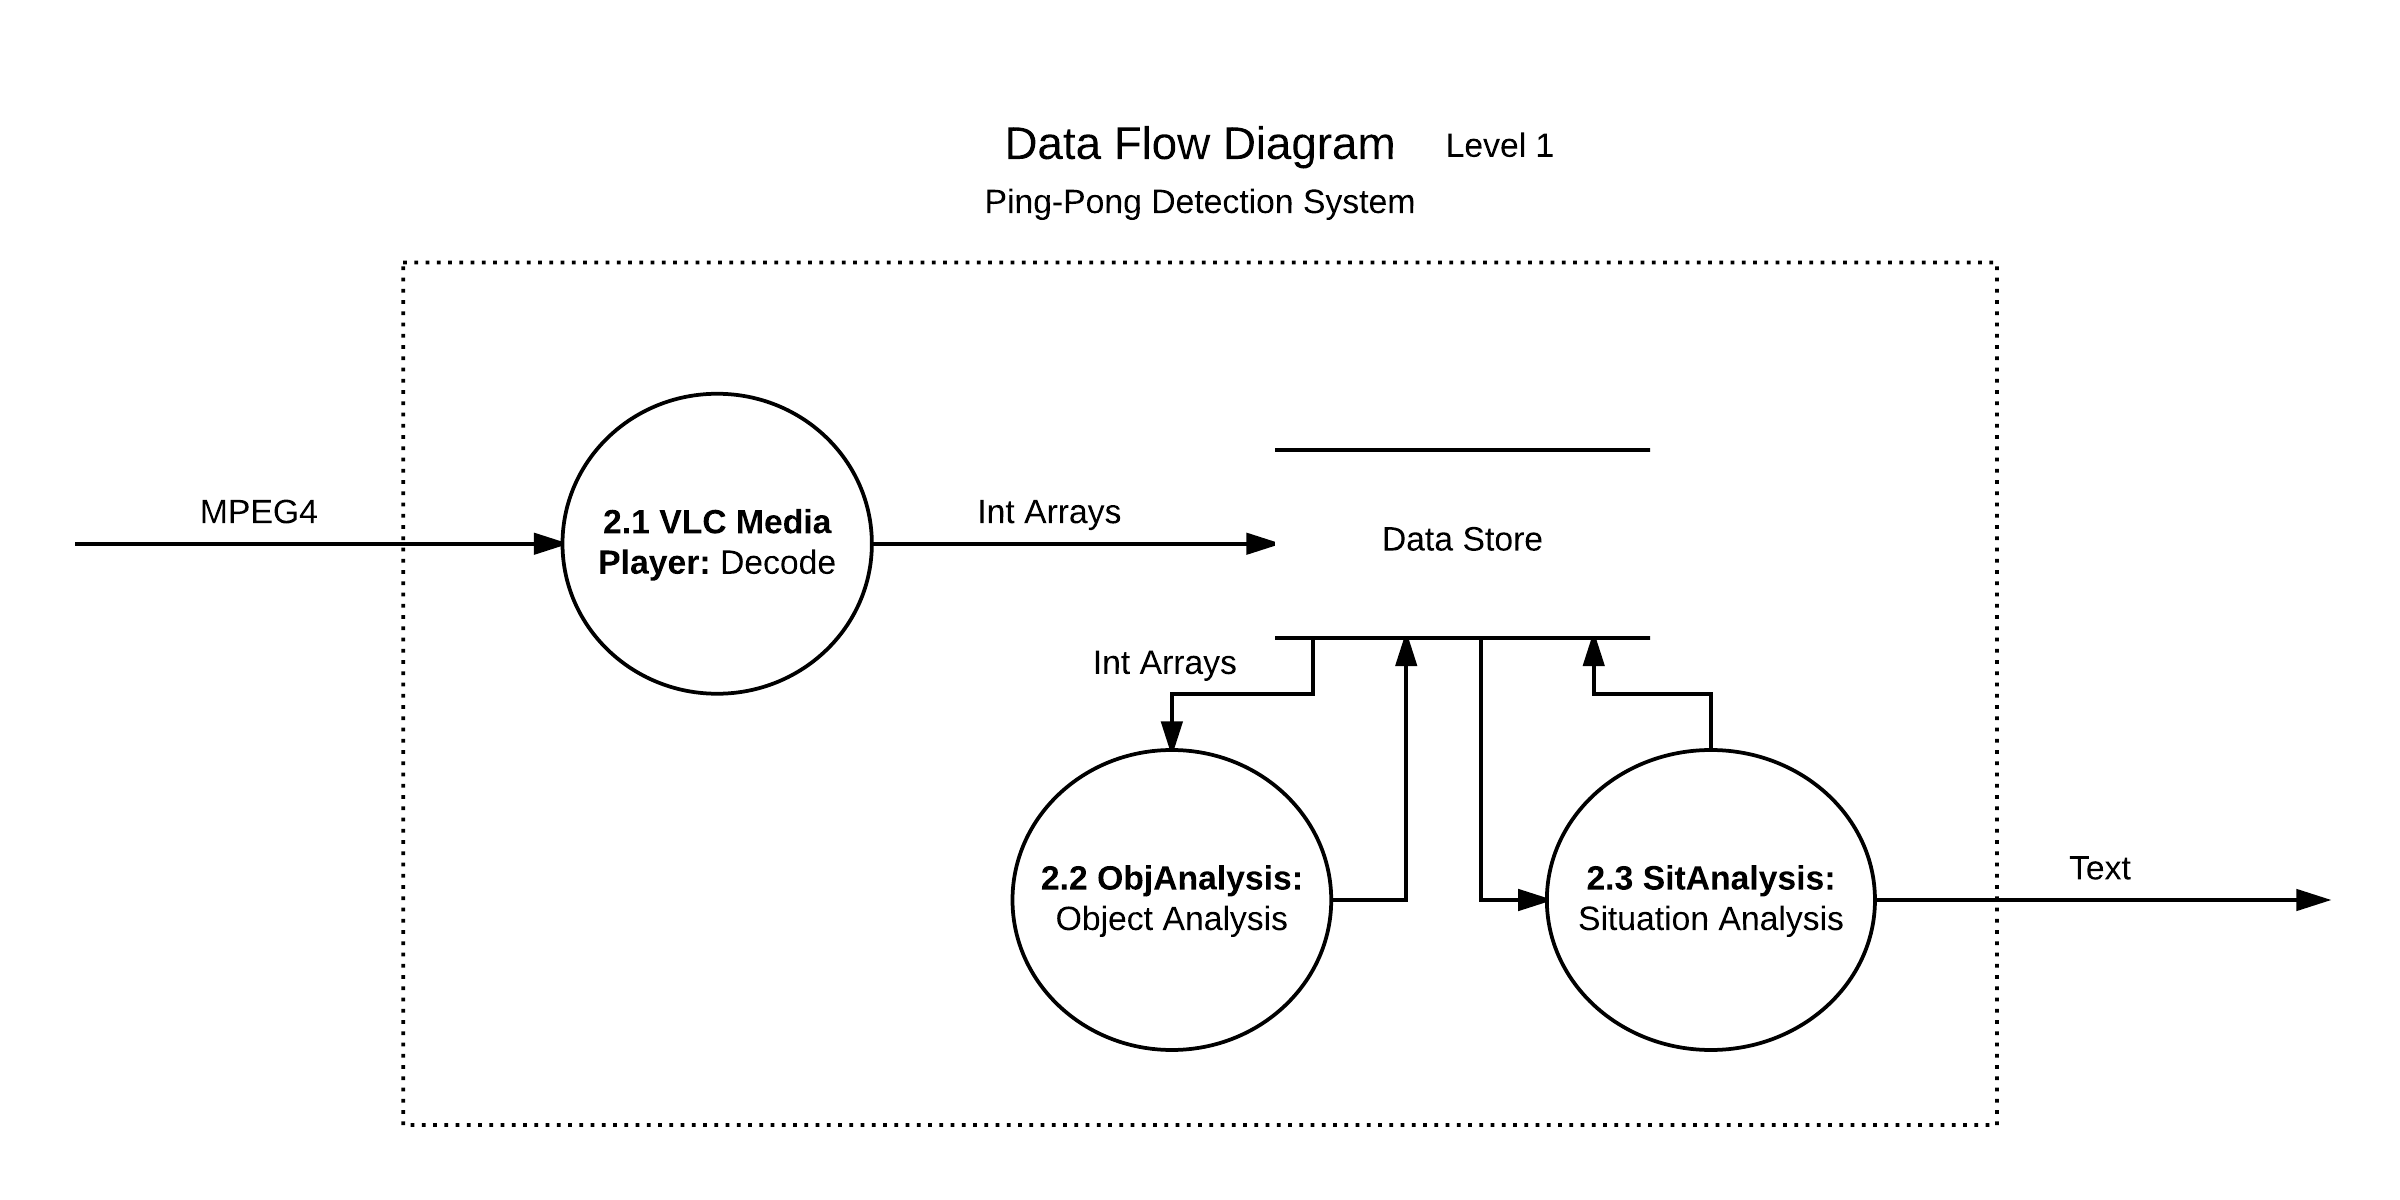
\includegraphics[width=1\textwidth]{Data-Flow-Level1.png}
\small{Data Flow Diagram: Level 1}
\end{center}
%\end{figure}
%%%%%%%%%%%%%%%%%%%%%%%%%%%%%%%%%%%%%%%%%
%\vspace{0.2cm}
Taking a closer look at the Ping-Pong Detection System process, we see that the frames of video are first decoded and then stored. The frames are then analyzed by the system for object analysis and stored again. Lastly, the system performs a situation analysis and once again stores the output, as well as sending the availability information text to the console.

\section{Non-functional Requirements}
The computer which runs our Ping-Pong Detection System (PDS) must have the following:\\
(1) Java 1.8 or greater\\
(2) VLC media player 2.1.x or greater (for 32 or for 64 bit systems, whichever matches the installed JVM)\\
(3) OpenCV libraries 2.4.9 or greater\\
(4) Access to the webcam transmitting video\\

\chapter{Design}

\begin{figure}[!h]
\begin{center}
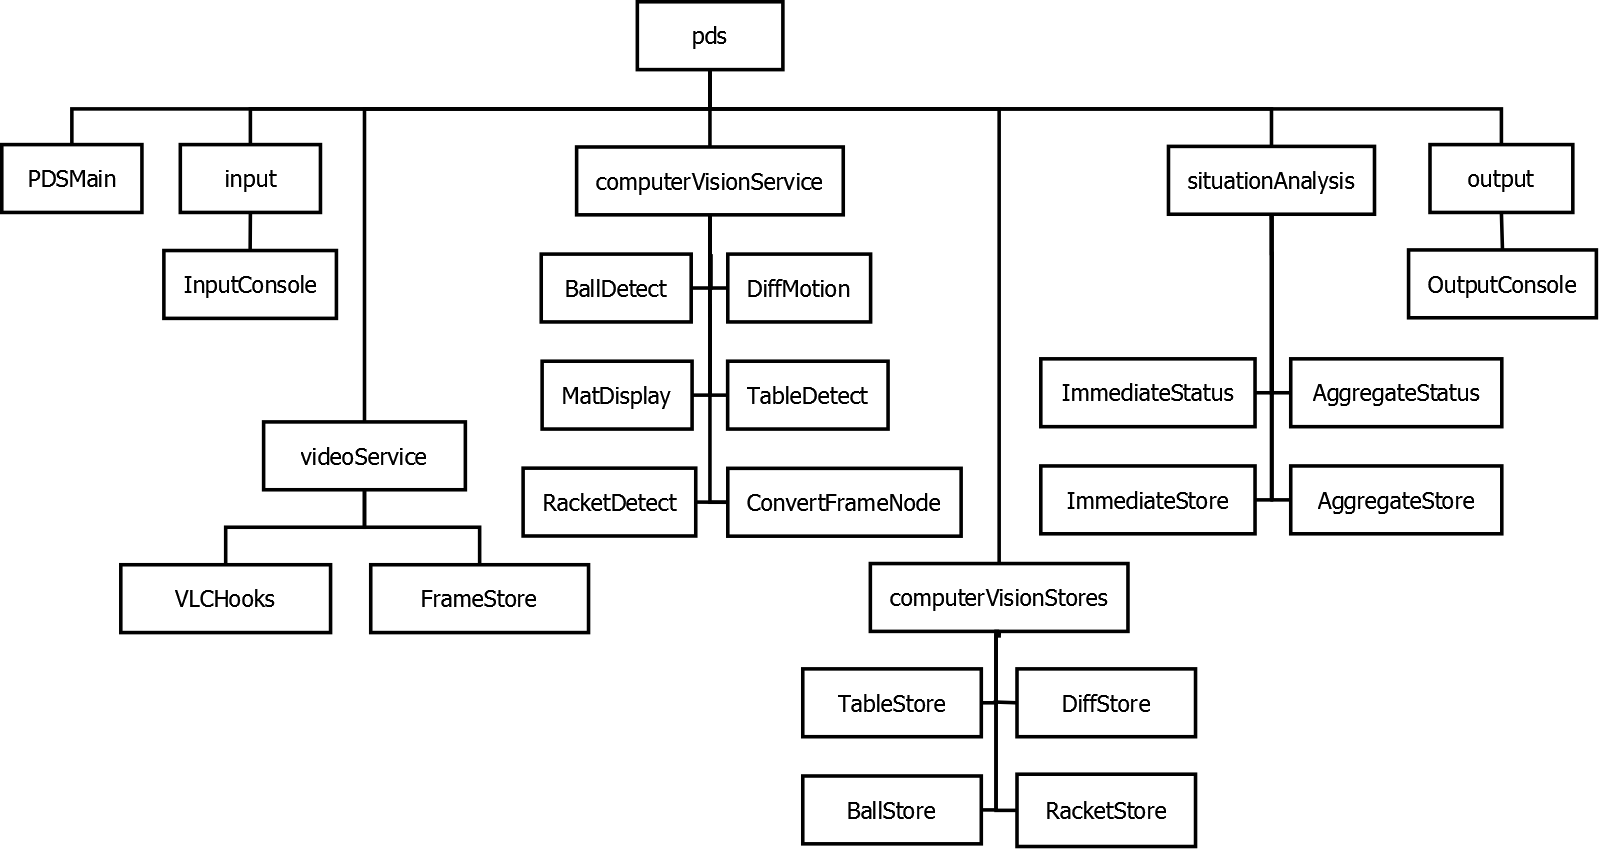
\includegraphics[width=1.05\textwidth]{Design-Comprises.png}
\end{center}
\caption{\small{COMPRISES Diagram}}
\label{fig:comprises}
\end{figure}

\section{Architecture}
\texttt{PDSMain}: This is the main program loop for the PDS program. It initializes all application threads, determines which jobs to launch for each frame, and ensures their synchronization where necessary.\\
Uses: all\\
\\
\texttt{videoService}: Decodes the video and provides frame data to the rest of the program.\\
Uses: none\\
\\
\texttt{computerVisionService}: Attempts to detect motion and objects (such as the table, ping pong ball, and ping pong rackets).  Provides locations to the program.\\
Uses: \texttt{videoService, computerVisionStores}\\
\\
\texttt{computerVisionStores}: Provides buffers which store \texttt{computerVisionService}'s location data.\\
Uses: none\\
\\
\texttt{situationAnalysis}: Analyzes the situation from object position data provided by \texttt{computerVisionStores} and decides what the ping pong table's current status is.\\
Uses: \texttt{computerVisionStores, output}\\
\\
\texttt{output}: Called by \texttt{situationAnalysis}, this module displays the ping-pong table status to the console.\\
Uses: none\\
\\
\texttt{input}: Receives a user's quit command and triggers a graceful exit.\\
Uses: none\\

\section{Design Rationale}
One thread will always be checking user \texttt{input} for a quit command, so this deserves its own module.  This allows changes to the way we perform the quit (for example, from a looping conditional to a message handler).  

Video decoding is a very different task domain, and so benefits being seperated into module \texttt{videoService}.  We also want our modules to perform comparisons between frames, for example, if calculating frame difference turns out to be a critical performance optimization.  Therefore \texttt{FrameStore} is its own submodule in \texttt{videoService} so the program can access frames after they've left the decoding buffer.

The team may also decide to switch what algorithms are used for tracking and detecting objects, so this makes \texttt{computerVisionService} appealing to break into its own module.  Similarly, deciding if the ping-pong table is in use or not requires its own set of algorithms and tweakable parameters.  Thus \texttt{situtationAnalysis} is its own seperate component.  The \texttt{computerVisionStores} module exists to give a common interface \verb'&' storage format for these modules' exchange of information.  Lastly, \texttt{output} is partitioned into its own module since it allows modifying specific wording of the output or the frequency without affecting our decision-making system.

\begin{figure}[H]
\begin{center}
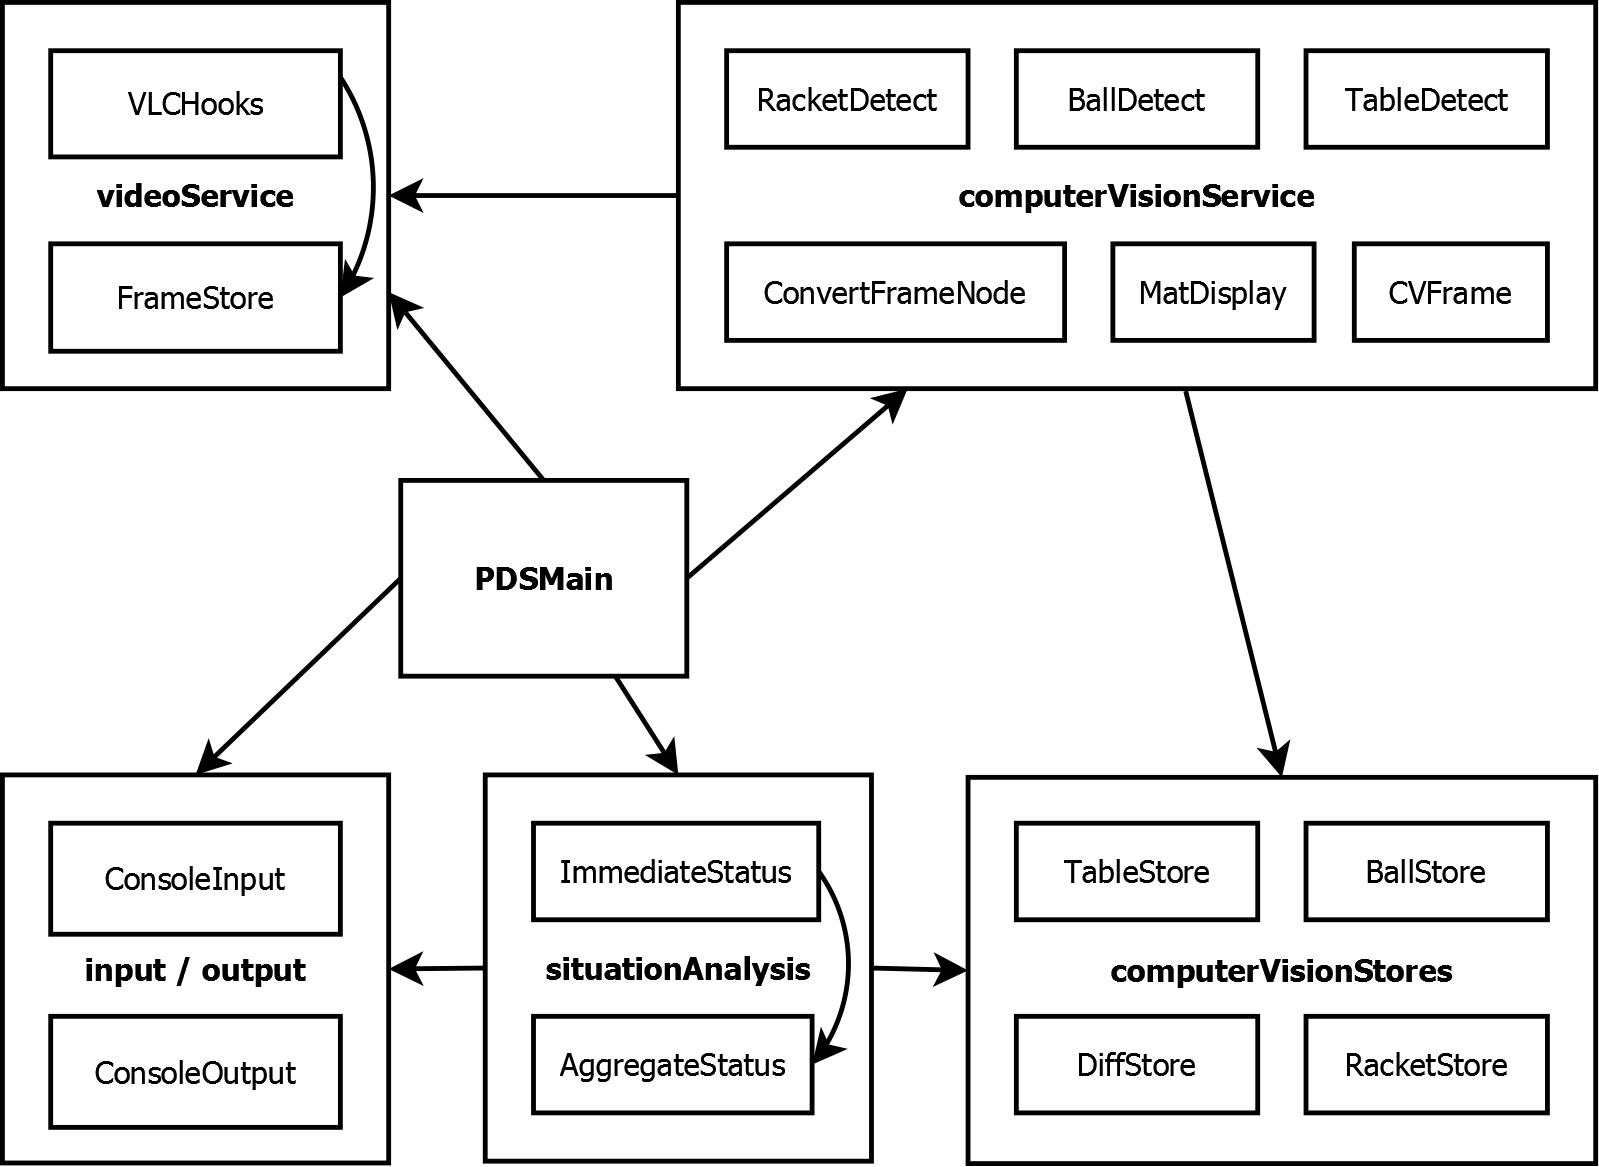
\includegraphics[width=1.05\textwidth,height=11cm,keepaspectratio]{Design-Uses.png}
\end{center}
\caption{\small{USES Diagram}}
\label{fig:uses}
\end{figure}

\section{Detailed Design}

\subsection{PDSMain}

This module is the thread controller, which consists of the main program loop and launches image processing tasks.  It uses \texttt{CountDownLatch}es to coordinate threads, and keeps the most recent two frames so that it can easily pass them to frame-comparative jobs.

\subsection{input}

Receives input from a user looking to terminate the program and triggers a graceful exit.  If the user enters input that is not the quit command, \texttt{input} will inform the user of the proper quit command.  This thread will run throughout the application's execution.  Component \texttt{main} will check the termination status periodically.\\
\\
Exports: \\
\texttt{boolean noQuitCommand()}

\subsection{videoService}

Hooks into the provided video decoding library and provides video frame data to the rest of the program.  The functionality hides behind the interface \texttt{VideoServiceIF}.  To decode video, the program currently uses software called VLC Player through the access library VLCJ.\\
\\
Exports: \\
\texttt{void startVideoService()}\\
\texttt{FrameStore getStorage()}

\subsubsection{FrameStore}

Storage and retrieval of raw frame data occurs here. To reduce latency, the buffer size has a maximum threshold after which older frames will be dropped.  Frames are provided as arrays rather than pixel-by-pixel for performance reasons.  An estimated 1 million pixel function calls for every still image in the video stream would severely impact real-time performance.  If no frames are available, null will be returned instead.\\
\\
Exports:\\
\texttt{FrameNode getFrame()}

\subsubsection{FrameNode}

This is the container for frame data, storing the aforementioned pixel array, the ID number of the frame, and the dimensions in pixels.  Frame numbers are stores as \texttt{long} to ensure the frame number will not wrap around to a negative number (not anytime in the creators' lifetimes, at least).\\
\\
Exports:\\
\texttt{int[] getData()}\\
\texttt{long getFrameNumber()}\\
\texttt{int getCols()}\\
\texttt{int getRows()}

\subsection{computerVisionService}

Attempts to detect objects such as the table, ping pong ball, and ping pong rackets.  Currently we use the OpenCV library to accomplish this.  Each computer vision algorithm can also run in its own thread for performance optimization.  Thus inputs and outputs are passed as construction parameters, and each class is \texttt{Runnable}.

\subsubsection{ConvertFrameNode}

This class converts frames from the VLC player-decoded format to the \texttt{Mat} format which OpenCV requires as input.  Depending on the needs of the computer vision algorithms, it can convert to color, grayscale, or black \& white.  It can also convert a frame to a binary edge-detected graphic.\\
\\
Exports:\\
\texttt{static Mat convertFrameNodeToCVi\_GRAY(FrameNode input)}

\subsubsection{DifferenceMotion}

\texttt{DifferenceMotion} calculates the overall motion between two frames.  It does so by summing the absolute average difference between pixels \texttt{x}, \texttt{y} in frame 1 and pixels \texttt{x}, \texttt{y} in frame 2.\\
\\
Exports:\\
\texttt{DifferenceMotion(CVFrame frame1, CVFrame frame2, DifferenceStore output, CountDownLatch semaphore)}

\subsubsection{TableDetect}

Tries to detect solid quadrilaterals within the image, with the goal of using these quadrilaterals to detect the presence or lack of the ping-pong table.  It uses a series of thresholds, magnifications, dialations, and edge detections from OpenCV.\\
\\
Exports:\\
\texttt{TableDetect(CVFrame frame, TableStore output, CountDownLatch semaphore)}

\subsubsection{BallDetect}

Attempts to detect the ball travelling over the table, apart from any other motion occuring in the video.\\
\\
Exports:\\
\texttt{BallDetect(CVFrame frame1, CVFrame frame2, BallStore output, CountDownLatch semaphore)}

\subsubsection{RacketDetect}

Uses a reference racket shape to fit any objects in the image.  To speed comparisons, the video image is first filtered by various OpenCV methods, reducing the candidate objects to be compared.

\subsection{computerVisionStores}

Provides locations and other per-frame or per-frame-comparison data (such as summed frame difference).  Consists of a store for each kind of visual analysis performed on the video.  Each store possesses a buffer with a constant \texttt{CAPACITY}, and when this is exceeded old values are dropped.  This is to save memory yet still allow the program to smooth sudden abberations in detection results.

\subsubsection{DifferenceStore}

Gives access to the computed frame-difference values.\\
\\
Exports:\\
\texttt{long getDifference(long frameNum)}\\
\texttt{boolean wasSkipped(long frameNum)}

\subsubsection{TableStore}

Stores the quadrilaterals which are potentially from lines on the table.\\
\\
Exports:\\
\texttt{ArrayList<MatOfPoint2f> getTableResults(long frameNum)}\\
\texttt{boolean wasSkipped(long frameNum)}

\subsubsection{BallStore}

Stores the potential ball candidates found with \texttt{BallDetect}.\\
\\
Exports:\\
\texttt{List<RotatedRect> getBoundingRectangles(Long frameNum)}

\subsubsection{RacketStore}

Stores the best racket-shape fit (0 is an exact fit, greater numbers deviate more) determined from each video frame.\\
\\
Exports:\\
\texttt{double getBestShapeFit(long frameNum)}

\subsection{situationAnalysis}

Analyzes the situation from object data provided by \texttt{computerVisionStores} and decides what the ping pong table's current status is.  This module looks not only at the immediate results, but also at an aggregation of the data.  This way a singular erroneous result should be smoothed out by taking the rest of the data into account.  Upon detecting a true change in status, it notifies the \texttt{output} module.

\subsubsection{ImmediateStatus}

This module converts the object data from \texttt{computerVisionStores} into a rough probability that a certain state is true (such as: the table is within the camera's view).  It then inserts this into an \texttt{ImmediateStore} buffer which it passes to \texttt{AggregateStatus} to perform a longer-range smoothed analysis.  \texttt{ImmediateStatus} itself runs as a thread so that these analyses do not delay the decoding and extraction of new video frames.\\
\\
Exports:\\
\texttt{ImmediateStatus(long frameNum, CVStores input, StatusStores output)\\
void run()}

\subsubsection{ImmediateStore}

Stores the rough probabilities calculated by \texttt{ImmediateStatus} and provides them to \texttt{AggregateStatus}.  The node class which it returns contains probabilities for the states that: 1) the table is available, 2) the table is in use, 3) the table is in the video frame, 4) there is motion in the video, and 5) the camera is encountering an error.\\
\\
Exports:\\
\texttt{ImmediateNode getProbabilities(long frameNum)}\\
\texttt{ImmediateNode [] getMultipleProbabilities(int count)}\\
\texttt{int getSize()}


\subsubsection{AggregateStatus}

Uses \texttt{ImmediateStore} (and potentially \texttt{computerVisionStore} in the future, if an edge case might arise) to determine the smoothed status over a length of several frames.  (The exact number of frames is set as a constant \texttt{SMOOTHING\_FACTOR}.)  The results are then placed in \texttt{AggregateStore} so that the main loop may access the results, which it needs in determining which computer vision jobs to launch.\\
\\
Exports:\\
\texttt{void parseImmedStatus()}


\subsubsection{AggregateStore}

Stores the final decisions made as to the status of the table.  Also includes variables which specifically store the last status which was decided, and the last frame that each status was detected.  Makes values available to the main loop and for future status calculations.\\
\\
Exports:\\
\texttt{enum GameStatus getGameStatus()}\\
\texttt{long getStatusFrameNum(enum GameStatus)}

\subsection{output}

Display simply reads the current status of the ping pong table and outputs it to the console.  Exact wording, insertion of a timestamp, and the method of output (console) are all controlled here.\\
\\
Exports: \\
\texttt{void printStatus(enum status)}

\chapter{Verification Plan}
\section{Verification Strategy}
\subsection{Black-box techniques}

\begin{table}[htbp]
\begin{center}
\begin{tabular}{|c|c|}\hline

Requirements&Tests\\\hline
CS1 & \tabincell{c}{ConsoleInputTest}\\\hline
CS2 & \tabincell{c}{ConsoleOutputTest}\\\hline
CS3 & \tabincell{c}{TableAvailableTest} \\\hline
CS6 & \tabincell{c}{TableAvailableTest} \\\hline
CS4 & \tabincell{c}{GameProcessTest}\\\hline
CS7 & \tabincell{c}{GameProcessTest}\\\hline
CS5 & \tabincell{c}{NoTableTest}\\\hline
CS9 & \tabincell{c}{RealTimeTest}\\\hline
G1 & \tabincell{c}{RealTimeTest}\\\hline
VR3 & \tabincell{c}{VideoServiceTest}\\\hline

\end{tabular}
\caption{The tests for requirements}
\end{center}
\end{table}

ConsoleInputTest: The ConsoleInputTest is used to test the requirement of CS1, the input of the console. When the user inputs the command to quit, the console will shut down.\\

ConsoleOutputTest: The ConsoleInputTest is used to test the requirement of CS2, the output of the console.\\

TableAvailableTest: Testing the requirement CS2 and CS5, which stand for the condition that ping pong table is available. When the testing results of these two requirements are ``The ping pong table is available",the tests are passed.\\

GameProcessTest: Testing the requirement CS3 and CS5, which are the situations that ping pong game is in process. When the testing results of CS3 and CS5 are ``Ping pong game is in process", the tests are passed.\\

NoTableTest: NoTableTest is the testing for CS4, in which condition there no longer exist a table in the video. When the testing result of CS4 is ``Camera is no longer pointing at the table", the test is passed.\\

RealTimeTest: RealTimeTest is used for testing the ability of real time of the project, as the requirements of CS8 and G1. When the project can change the appropriate message as soon as the new statue is detected, the test is passed.\\

VideoServiceTest: VideoServiceTest is used to test the performance of video decoding.

\subsection{Video Tests}

Due to the application's real-time nature, much testing will necessarily involve non-automated processes.  For one, automated video testing would increase the time to perform tests by several minutes at each commit, since the application decodes strictly in real-time and uses interval-based smoothing to iron out anamalous signals (such as a video frame corrupted in transmission).  Therefore, several test videos have been made from the samples provided by Scott Kay.  These are available at \url{http://cisc475-2.cis.udel.edu/testvids/} and test the following cases:\\
\\
\begin{table}[htbp]
\begin{center}
\begin{tabular}{|c|}\hline
\textbf{Test Cases}\\\hline
Free to In-Use\\\hline
In-Use with Long Gap\\\hline
In-Use to Free with Rackets\\\hline
No Table with Motion\\\hline
Little Table with Little Motion\\\hline
\end{tabular}
\caption{Video Tests}
\end{center}
\end{table}

\subsection{White-box techniques}
For white-box techniques, we will use Jacoco for our project. And for each module, statement coverage and branch coverage will be done. The statement coverage need to achieve 100 percent. 
Moreover, we expect the branch coverage to get 60 percent to 70 percent.


\subsection{Testing  at different levels}
1. Unit testing plan\\
Unit testing plan shown in table 4.3\\
Please note that we are unable to write tests that pass on the headless UDel virtual machine for class \texttt{VLCHooks} due to its invocation of GUI elements necessary for VLC Player decoding interface. These same tests pass successfully in a GUI environment.
\begin{table}[htbp]
\begin{center}
\begin{tabular}{|c|c|c|c|}\hline
Packages & Classes & Unit Tests & Stubs\\\hline    
pds&\tabincell{c}{PDSMain}& \tabincell{c}{PDSMainTest}&\tabincell{c}{}\\\hline
pds.computerVisionService& \tabincell{c}{ConvertFrameNode\\CVStores\\Lines\\LineStore\\BallDetect\\DiffMotion\\DiffStore}&\tabincell{c}{ CoverFrameNodeTest\\ CVStoresTest \\LineTest} &\tabincell{c}{ DiffMotionStub\\DiffStoreStub\\LineStoreStub}\\\hline
pds.input  &\tabincell{c}{ConsoleInput}& \tabincell{c}{ConsoleInputTest}& \tabincell{c}{} \\\hline
pds.output  &\tabincell{c}{ConsoleOutput}& \tabincell{c}{CosoleOutputTest}&\tabincell{c}{} \\\hline
pds.situationAnalysis  &\tabincell{c}{AggregateStatus\\AggregateStore\\ImmediateStatus\\ImmediateStore}&\tabincell{c}{}&\tabincell{c}{ AggregateStatusStub\\AggregateStoreStub\\ ImmediateStatusStub\\ImmediateStoreStub}\\\hline
pds.videoService&\tabincell{c}{FrameNode\\FrameStore\\VideoServiceIF\\VLCjVideoService\\EXLUDING VLCHooks} &\tabincell{c}{ VideoServiceTest } &\tabincell{c} {FrameStoreStub}\\\hline

\end{tabular}
\caption{Unit Testing Plan}
\end{center}
\end{table}
\\
2. Integration testing plan
The order of integration testing plan is shown in Figure 4.1\\
(1)The first two modules we need to test are VLCHooks module and FrameStore module. After they pass tests, the videoService should too be tested.\\
(2)After test DiffMotion, Lines, VectorMotion and Objects, these four modules can integrate to test the module of computerVisionService.\\
(3)AggregateStatus and ImmediateStatus should to be tested in order before we integrate them to test situationAnalysis.\\
(4)computerVisionStores can be tested after all the submodules are passed.\\
\\
3. System testing
System testing will be done after the integration testing. The whole system shows on Figure 3.2. Make sure the whole system works, we need to test whether the system can realize the requirements, so that a lot of different videos are required.\\
\\
4. Acceptance testing
After the system testing is passed, we will deliver the project to the client to do the acceptance testing. 

%%%%%%%%%%%%%%%%%%%%%%%%%%%%%%%%%%%%%
\begin{figure}[htb]
\centering
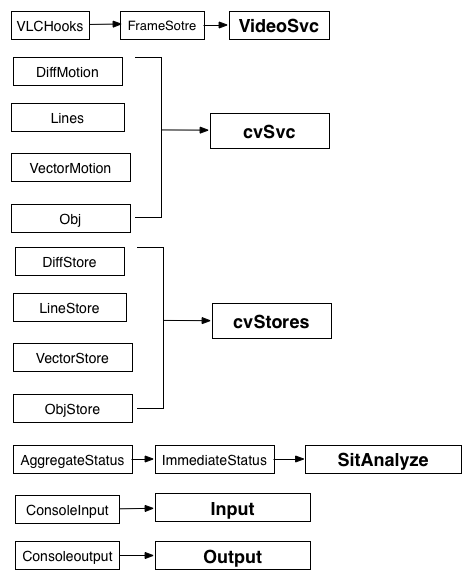
\includegraphics[width=0.6\textwidth]{integration.png}
\caption{ \small{Integration Plan}}
\end{figure}
%%%%%%%%%%%%%%%%%%%%%%%%%%%%%%%%%%%%%

\section{Challenges for testing}
1. Testing a particular case, we need to prepare a short video for it. However, although the test is passed, we cannot sure the system can deal with the actual video. There are a lot of differences between two videos, such as the position o table or the angle of camera. Therefore, we need to prepare several different videos to test one case. \\
\\
2.  As we do testing on different level, there is not a actual value we can test. As unit testing `LinesTest' for example, this class doesn't have an actual return value, it just return a line, its start point and end point. Moreover, for different video, the returns are also different. Therefore, how to test these class is a challenge.

\section{Status of testing}
\subsection{The status of black-box testing}

\begin{table}[H]
\begin{center}
\begin{tabular}{|c|c|}\hline
Black-box tests &Status \\\hline
ConsoleInputTest & \tabincell{c}{passed} \\\hline
ConsoleOutputTest & \tabincell{c}{passed} \\\hline
TableAvailableTest& \tabincell{c}{not written yet} \\\hline
GameProcessTest& \tabincell{c}{not written yet}\\\hline
NoTableTest & \tabincell{c}{not written yet}\\\hline
RealTimeTest & \tabincell{c}{not written yet}\\\hline
VideoServiceTest & \tabincell{c}{passed}\\\hline
\end{tabular}
\caption{The status of Black-box testing}
\end{center}
\end{table}

\subsection{The status of unit testing}

\begin{table}[H]
\begin{center}
\begin{tabular}{|c|c|}\hline
Unit tests & Status \\\hline
PDSMainTest & \tabincell{c}{passed*} \\\hline
CoverFrameNodeTest &\tabincell{c}{passed}\\\hline
CVStoresTest & \tabincell{c}{passed}\\\hline
LineTest& \tabincell{c}{passed}\\\hline
ConsoleInputTest & \tabincell{c}{passed}\\\hline
CosoleOutputTest& \tabincell{c}{passed}\\\hline
VideoServiceTest & \tabincell{c}{passed}\\\hline
\end{tabular}
\caption{The status of unit testing}
\caption*{ *One test in \texttt{PDSMainTest} is not passing on the UDel virtual machine due to the machine's headless nature and our program's need to initialize GUI elements, but this test does pass in a GUI environment.}
\end{center}
\end{table}


\appendix

\chapter{Glossary}

%\gloss{modularity}{the quality of being divided into modules.  I will
  %continue this definition just because I want to see what it looks
  %like when it wraps around a line.  Not too shabby, if I do say so
  %myself.}

\gloss{DFD}{Data Flow Diagrams show the flow of data through the system.}

\gloss{ERD}{Entity-Relationship Diagrams show relationships among entities.}

\gloss{frame}{A video is composed of many still images, called frames, which are displayed at a rapid rate to appear as a moving scene.}

\gloss{GPU}{A Graphics Processing Unit, which aids some computers in rendering 3D and 2D graphical content.}

\gloss{GUI}{Graphical user interface, such as Windows.  This is in contrast to a textual command line terminal.}

\gloss{MPEG2/MPEG4}{Two related standards for lossy compression of video content.}

\gloss{PDS}{PDS is short for Ping-Pong Detection System, the name of the project.}

\gloss{VLC}{VLC media player(VLC) is a portable, free and open-source and streaming media player, which is used by the project to recieve and decode video.  Importantly, VLC is capable of decoding the MPEG2/MPEG4 formats.}

\gloss{VLCJ}{The library of VLC for java}

\begin{thebibliography}{1}

\bibitem{source1} \url {http://vlc-player.downloadape.org/about}
  
\end{thebibliography}


\end{document}

